\section{Распределённое тестирование решений}

Автоматическое тестирование представляет собой запуск решения на заранее подготовленных тестах и проверку ответа на каждом тесте.
Решение пользователя может быть написано на одном из разрешённых языков программирования (Python, C++, Go).
Некоторые из языков подразумевают предварительную компиляцию кода и запуск двоичного кода.
Проверка ответа выполняется с помощью чекера --- специальной программы,
которая также может быть реализована на одном из разрешённых языков программирования.

Процесс тестирования решения может быть представлен в виде ориентированного ацикличного графа,
вершинами которого являются атомарные команды (например, компиляция кода или запуск кода на одном тесте),
а ребро проводится из вершины A в вершину B, если выполнение команды B требует артефакты выполнения команды A.

Exesh предоставляет для использования несколько типов Job (команд):
\begin{itemize}
\item компиляция C++ кода;
\item компиляция Go кода;
\item запуск бинарного файла;
\item запуск Python кода;
\item запуск бинарного файла чекера.
\end{itemize}

На основе метаданных задачи и языка программирования решения компонент Taski формирует Execution ---
описание процесса тестирования в виде графа Jobs --- и отправляет его в Exesh для выполнения.
Добавление поддержки нового языка программирования требует лишь добавления нового типа Job в Exesh.
Добавление нового формата задачи требует добавления новой стратегии формирования Execution в Taski.
Далее процесс тестирования рассматривается как выполнение Execution, представляющего собой ориентированный ацикличный граф Jobs.

Так как не все Jobs в Execution зависят друг от друга последовательно, некоторые можно выполнять параллельно.
Пример параллельного исполнения графа Jobs показан на рисунке \ref{execution-graph}.
На нём разными цветами отмечены Jobs, которые могут быть выполнены на разных workers.
Такой подход позволяет эффективно использовать вычислительные ресурсы и сокращать суммарное время тестирования решений.

\begin{figure}[ht]
\begin{center}
\scalebox{0.6}{
   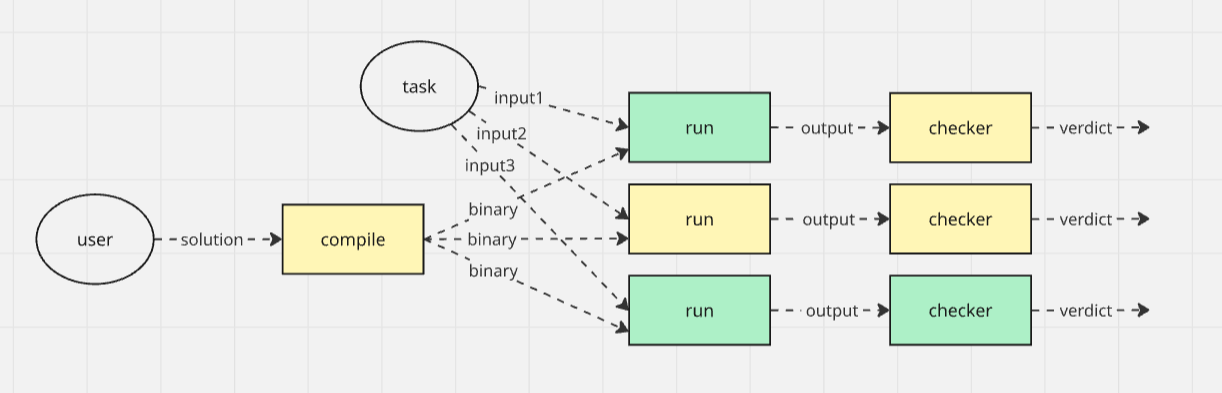
\includegraphics{images/execution-graph.png}
}
\caption{
\label{execution-graph}
     Пример распределённого исполнения Execution.}
\end{center}
\end{figure}

\subsection{Распределение ресурсов для исполнения набора Execution}

Пусть в момент времени $t$ система исполняет набор из $N$ Executions.
Пусть каждый Execution содержит $K_i$ Jobs ($i = 1, 2, \dots, N$).
Пусть каждый Job имеет ожидаемое время выполнения $time_{i, j}$ ($i = 1, 2, \dots, N$, $j = 1, 2, \dots, K_i$).
Оценка ожидаемого времени выполнения Job осуществляется при помощи статистических данных.
Используется предположение, что пользовательские решения на конкретном тесте в конкретной задаче имеют близкое время выполнения.

При последовательном выполнении всех Jobs в $i$-м Execution требуется $total_i = \sum_{j = 1}^{K_i} time_{i, j}$ времени.
Система имеет набор Workers, что позволяет исполнять Jobs параллельно и уменьшать реальное время исполнения Execution.
Пусть $i$-й Execution начал исполнение во время $start_i$.
Тогда в момент времени $t$ реальное время исполнения $i$-го Execution составляет $t - start_i$.

Задача заключается в выборе Execution, из которого должен быть выбран следующий Job для выполнения.
Иллюстрация задачи изображена на рисунке \ref{executions-problem}.

\begin{figure}[ht]
\begin{center}
\scalebox{0.4}{
   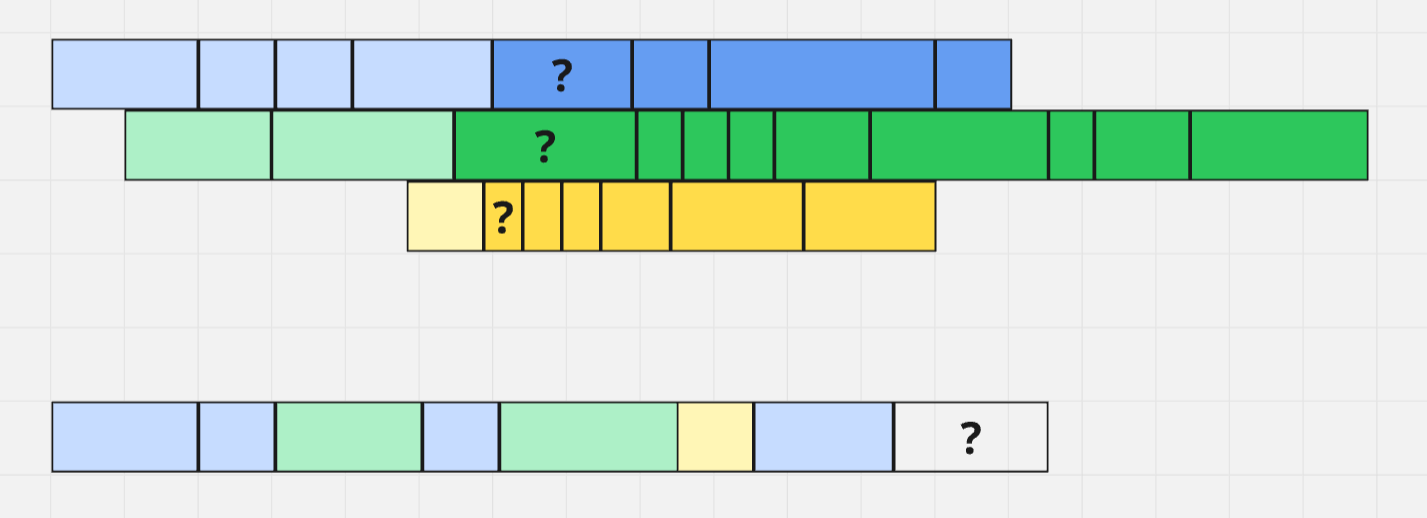
\includegraphics{images/executions-problem.png}
}
\caption{
\label{executions-problem}
     Задача выбора Execution для исполнения.}
\end{center}
\end{figure}

Введём функцию $priority(i, t)$ --- приоритет исполнения $i$-го Execution в момент времени $t$.
Подход заключается в сортировке Executions по их приоритету и выборе наиболее приоритетного Execution.

Рассмотрим, что должно влиять на приоритет Execution.
Во-первых, хочется, чтобы Execution, находящийся в системе дольше, получал больше ресурсов.
То есть приоритет должен зависеть от реального времени исполнения Execution.

Однако, если каждый раз выбирать самый старый живой Execution,
то получится так, что новые Executions не будут получать ресурсы, пока не закончат исполнение все ранее созданные.
Поэтому, во-вторых, на приоритет Execution должен влиять текущий прогресс исполнения.
Чем меньше ресурсов в относительном отношении получал Execution ранее, тем больше должен быть его приоритет.
Пусть в данный момент времени в $i$-м Execution были выполнены первые $F_i$ Jobs.
Прогресс должен быть рассчитан, исходя из ожидаемого времени выполнения Jobs,
поэтому для $i$-го Execution он будет равен $done_i = \sum_{j = 1}^{F_i} time_{i, j}$.

Также стоит сделать акцент на том, что разные Executions имеют разное суммарное ожидаемое время исполнения,
поэтому при подсчёте приоритета нужно использовать не абсолютное, а относительное время, зависящее от размера Execution.
Приоритет определяется следующим образом:

\begin{equation}
   priority(i, t) = \left(\frac{t - start_i}{total_i} + \alpha \cdot \frac{total_i - done_i}{total_i}\right) \times \gamma^{tries_i - 1}
\end{equation}

Формула содержит два основных компонента --- реальное время исполнения и ожидаемое время до конца исполнения.
Они по-разному должны влиять на приоритет, поэтому был введён параметр $\alpha$, определяющий отношение их влияния на приоритет.
Во время исполнения Execution может произойти ошибка (например, падение Coordinator).
В таком случае Execution будет перезапущен, но его приоритет при повторном запуске должен быть повышен.
Пусть $tries_i$ --- количество попыток выполнения $i$-го Execution,
тогда приоритет будет экспоненциально зависеть от этого значения и параметра $\gamma$.
Таким образом, приоритет увеличивается с ростом времени жизни Execution, при уменьшении доли уже выполненной работы,
а также при повторных запусках Execution после ошибок.

\subsection{Эффективное распределение Jobs по исполнителям}

Каждый worker в кластере имеет в своём распоряжении $S$ слотов.
Для выполнения одного Job требуется один слот на время выполнения Job.
Будем считать, что один слот соответствует $1$ CPU и $256$ MB RAM.
При этом Job может использовать больше $256$ MB RAM, но должно быть выполнено ограничение,
что в любой момент времени количество Jobs, выполняемых на worker, должно быть не более $S$,
а также что суммарный объём используемой памяти всеми выполняемыми Jobs должно не превышать $256 \cdot S$.

Пусть каждый Job имеет ожидаемый объём используемой памяти $memory_{i, j}$ ($i = 1, 2, \dots, N$, $j = 1, 2, \dots, K_i$).
Оценка ожидаемого объёма используемой памяти Job осуществляется при помощи статистических данных.
Используется предположение, что пользовательские решения на конкретном тесте в конкретной задаче имеют близкие значения памяти.

Каждый Job можно представить в виде прямоугольника с размерами $time \times memory$
на плоскости, в которой по оси Ox откладывается время, а по оси Oy --- память.
Для выполняемого Job ставится прямоугольник с левой стороной по координате начала выполнения,
и с правой стороной по ожидаемому окончанию выполнения.
В каждый момент времени любая прямая, параллельная оси Oy, должна пересекать не больше $S$ прямоугольников.

Рассмотрим очередной heartbeat-запрос от одного worker.
Нужно выбрать один Job, который отдать на выполнение этому worker.
Каждый worker имеет множество выполняемых в данный момент Jobs.
Имеется последовательность Executions, упорядоченная по приоритету, а каждый Execution предоставляет для выполнения один Job.

Простой алгоритм заключается в том, чтобы выбрать Job из самого приоритетного Execution и отдать его на выполнение.
Однако, такой алгоритм может неэффективно использовать ресурсы системы.
Пример проиллюстрирован на рисунке \ref{jobs-problem}.

\begin{figure}[ht]
\begin{center}
\scalebox{0.4}{
   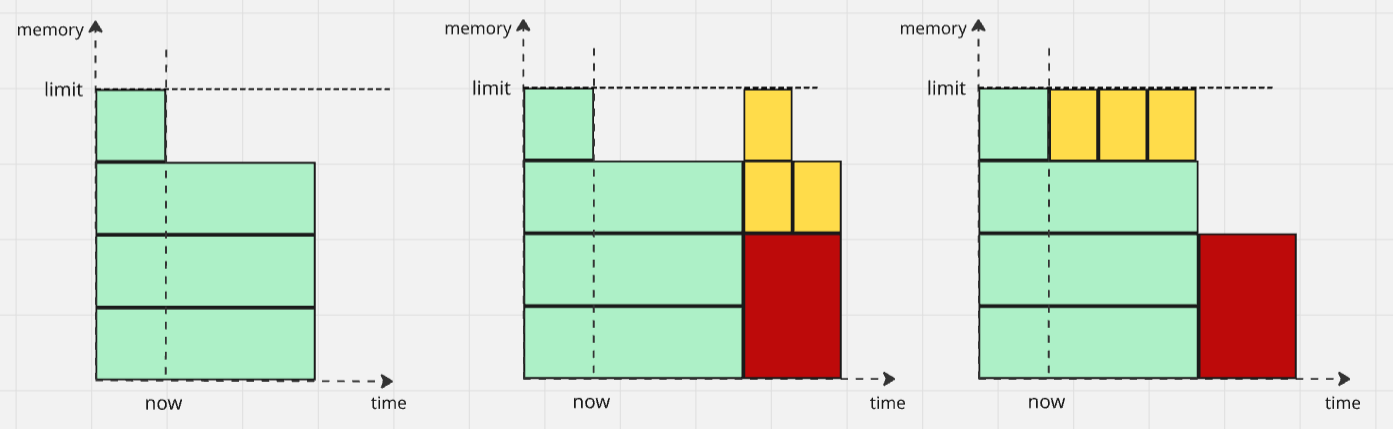
\includegraphics{images/jobs-problem.png}
}
\caption{
\label{jobs-problem}
     Задача распределения вычислительных ресурсов кластера.}
\end{center}
\end{figure}

Предположим, что в текущий момент времени есть большой более приоритетный Job (красного цвета)
и несколько маленьких менее приоритетных Jobs (жёлтого цвета).
Алгоритм, который всегда выбирает Job из наиболее приоритетного Execution,
в момент текущий момент времени не может отдать на выполнение красный Job, и ему приходится ждать окончания уже выполняемых Jobs.
Однако, эффективный способ утилизации ресурсов заключается в том,
что можно выполнить менее приоритетные жёлтые Jobs перед более приоритетным красным,
и этом ожидаемое время начала выполнения более приоритетного Job не изменится,
что позволяет повысить утилизацию ресурсов без ухудшения работы предыдущего алгоритма.

Псевдокод promise-based алгоритма выглядит следующим образом:

\begin{minted}{python}
def schedule(jobs, promised_jobs):
   for job in promised_jobs:
      if can_start_now(job):
         start(job)
         return
   
   jobs.sort(key=job.priority)

   for job in jobs:
      if can_start_now(job):
         start(job)
         return
      elif len(promised_jobs) < limit:
         start_time = get_start_time(job)
         promise(job, start_time)
\end{minted}

Суть алгоритма заключается в том, что он пытается понять, может ли запустить сейчас самый приоритетный Job,
и если может, то запускает, а если нет, то вычисляет минимальное возможное время начала и резервирует его.
Когда возникает очередная возможность запустить Job, алгоритм сначала пытается запустить promised Jobs,
а если не получается, то пытается запустить остальные в порядке приоритета.
Алгоритм использует две основные функции:
\begin{itemize}
\item can\_start\_now(job) --- можем ли сейчас запустить job, не нарушив существующие резервации;
\item get\_start\_time(job) --- минимальное время, в которое получится запустить job, не нарушив существующие резервации.
\end{itemize}

Алгоритм принимает решения, используя только текущую информацию о выполняемых Jobs и статистические оценки ресурсов,
поэтому вводится ограничение на максимальное количество promised Jobs,
чтобы не происходило деградации планировщика из-за большого количества зарезервированных Jobs.

\subsection{Исполнение команд в изолированном окружении}

Исполнение команд предполагает запуск произвольного пользовательского кода в системе.
Это может повлечь серьёзные последствия для инфраструктуры платформы, если не вводить ограничения на действия пользовательского кода.

При выполнении пользовательского кода необходимо ограничивать следующие возможности:
\begin{itemize}
\item доступ к файловой системе вне рабочей директории;
\item взаимодействие с сетевым интерфейсом;
\item создание новых процессов и потоков;
\item превышение использования процессорного времени и оперативной памяти;
\item выполнение потенциально опасных системных вызовов.
\end{itemize}

Также необходимо ограничивать время выполнения и объём используемой памяти.
Измерение должно производиться по времени исполнения процесса на процессоре, а не по реальному времени,
что позволяет избежать ошибок, вызванных конкурентным выполнением других процессов,
и обеспечить повторяемость результатов независимо от текущей нагрузки системы.

Для запуска пользовательского кода была выбрана утилита isolate,
которая разработана специально для использования в системах автоматического тестирования решений.
Утилита использует механизмы изоляции процессов Linux, такие как namespaces и cgroups,
что позволяет ограничивать доступ программы к системным ресурсам и изолировать процессы друг от друга.

Выбор isolate вместо разработки собственной системы изоляции процессов был обусловлен
её широким использованием в системах автоматического тестирования решений (например, на IOI),
что является хорошим подтверждением надёжности утилиты, а также низкими накладными затратами на использование.
По сравнению с реализацией на основе Docker-контейнеров, isolate позволяет уменьшить время запуска команд,
что особенно важно при большом количестве короткоживущих процессов тестирования.

\subsection{Подход к взаимодействию с файловой системой}

Для взаимодействия с файловой системой в компонентах Taski и Exesh используется библиотека filestorage,
которая была написана специально для этого проекта и поддерживает эффективный и конкурентный доступ к ресурсам системы.

Библиотека оперирует понятием бакет --- независимая единица разделения файловой системы.
Бакет является папкой, которая может содержать другие папки и файлы, но не бакеты.
Каждый бакет имеет уникальный идентификатор, представляющий собой SHA-1 хеш длиной 20 байт (40 hex-символов).
Бакеты разделяются на 256 шардов (по первым двум hex-символам идентификатора), каждый из которых лежит в отдельной папке.
Такое разделение уменьшает количество объектов внутри одной директории и повышает эффективность работы с файловой системой.
Каждый бакет имеет время жизни либо является бессрочным.
Библиотека поддерживает автоматическое удаление бакетов по истечении их времени жизни.

Библиотека позволяет передавать бакеты и отдельные файлы между компонентами системы.
Передача ресурсов осуществляется в формате tar-stream с использованием сжатия.
Ресурсы сначала скачиваются во временную папку, а затем переносятся в основное хранилище.
Интерфейс библиотеки предоставляет методы commit и abort, которые влияют на перенос ресурсов в основное хранилище из временного.
Если бакет или файл уже присутствует в локальном хранилище, повторная загрузка не выполняется.

\subsection{Нагрузочное тестирование системы}

Для нагрузочного тестирования был использован сервер с конфигурацией $8$ CPU с тактовой частотой $3.3$ ГГц и $8$ ГБ RAM.
На сервере были развёрнуты компоненты Duely, Analyzer, Taski, Exesh и Dashboard.
В Exesh был кластер с двумя workers и одним coordinator.
Каждый worker имеет возможность одновременно исполнять $4$ Jobs, то есть всего одновременно может исполняться $8$ Jobs.

Предполагалось, что компонентами системы суммарно будет использоваться $1$ CPU,
а остальные $7$ CPU будет выделено планировщиком операционной системы для запуска пользовательского кода.
Производился запуск трёх наборов по пять Executions, между которыми был отступ $5$ секунд.
Между Executions в одном наборе был случайный отступ от $1$ до $3$ секунд.
Все Executions содержали по $50$ Jobs, каждый из которых выполняется $1$ секунду.

Если производить последовательный запуск всех Jobs на одном CPU, то потребуется $1 \cdot 50 \cdot 15 = 750$ секунд.
В результате нагрузочного тестирования было определено,
что между началом первого Execution и окончанием последнего проходит $105$ секунд.
Таким образом, параллельная обработка на $8$ CPU происходит в $7.14$ раз быстрее, чем последовательная на одном CPU.
Результат оказался вполне достойным --- компонентами системы суммарно использовалось даже меньше $1$ CPU,
а все остальные ресурсы были выделены для запуска пользовательского кода.
В то же время, при увеличении количества CPU выделение ресурсов для компонентов системы растёт не так быстро,
и эффективность параллельного исполнения приближается к количеству CPU.

Также проводилось тестирование разных алгоритмов подсчёта приоритета Execution.
Были рассмотрены формулы, которые учитывают только реальное время исполнения, только ожидаемое оставшееся время исполнения,
а также учитывающие оба фактора, но с разными значениями коэффициента $\alpha$.
Для сравнения были выбраны графики, иллюстрирующие изменение приоритета и прогресса Execution.

Графики, получившиеся при расчёте приоритета, исходя только из реального времени исполнения ($\alpha = 0$),
изображены на рисунках \ref{priority_alpha-0} и \ref{progress_alpha-0}.
Видно, что приоритеты растут линейно и следующий Execution не начинают исполнение до окончания предыдущего.

\begin{figure}[ht]
\begin{center}
\scalebox{0.3}{
   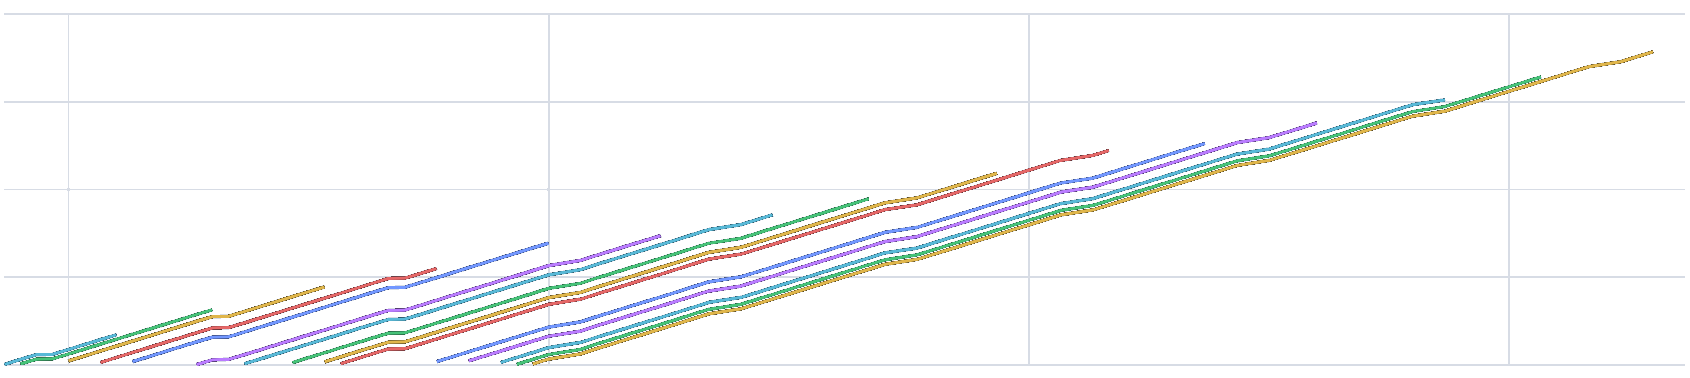
\includegraphics{images/executions/priority_alpha-0.png}
}
\caption{
\label{priority_alpha-0}
     Изменение приоритетов при $\alpha = 0$.}
\end{center}
\end{figure}

\begin{figure}[ht]
\begin{center}
\scalebox{0.3}{
   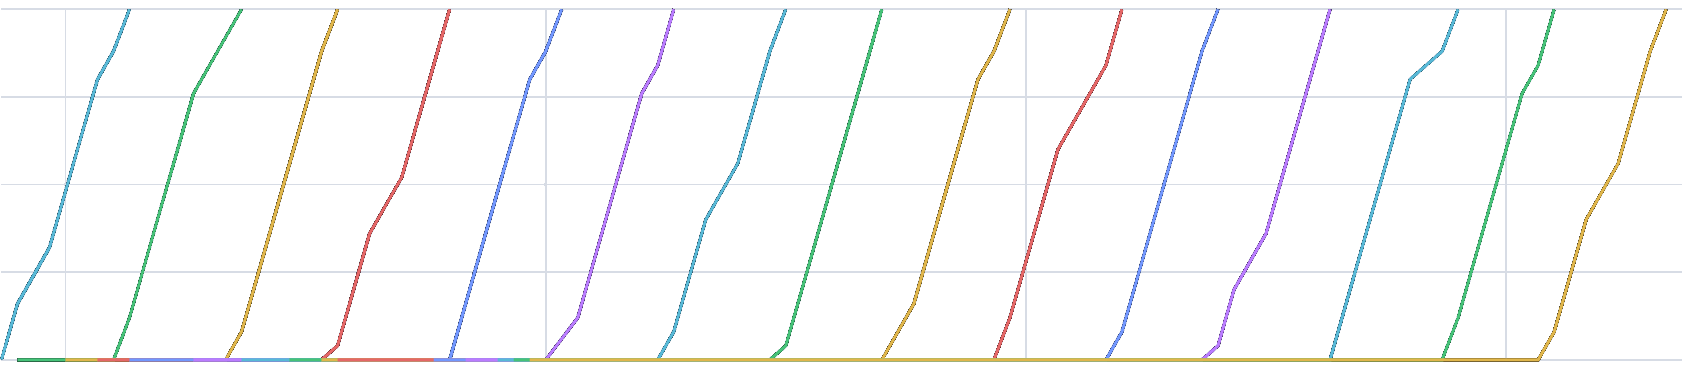
\includegraphics{images/executions/progress_alpha-0.png}
}
\caption{
\label{progress_alpha-0}
     Изменение прогрессов при $\alpha = 0$.}
\end{center}
\end{figure}

Графики, получившиеся при расчёте приоритета, исходя только из ожидаемого оставшегося времени исполнения ($\alpha \to \infty$),
изображены на рисунках \ref{priority_alpha-inf} и \ref{progress_alpha-inf}.
Видно, что приоритеты уменьшаются с течением времени, а также что в какой-то момент все приоритеты выравниваются,
и остаются таковыми до конца исполнения всех Executions, которые заканчивают исполнение одновременно.

\begin{figure}[ht]
\begin{center}
\scalebox{0.3}{
   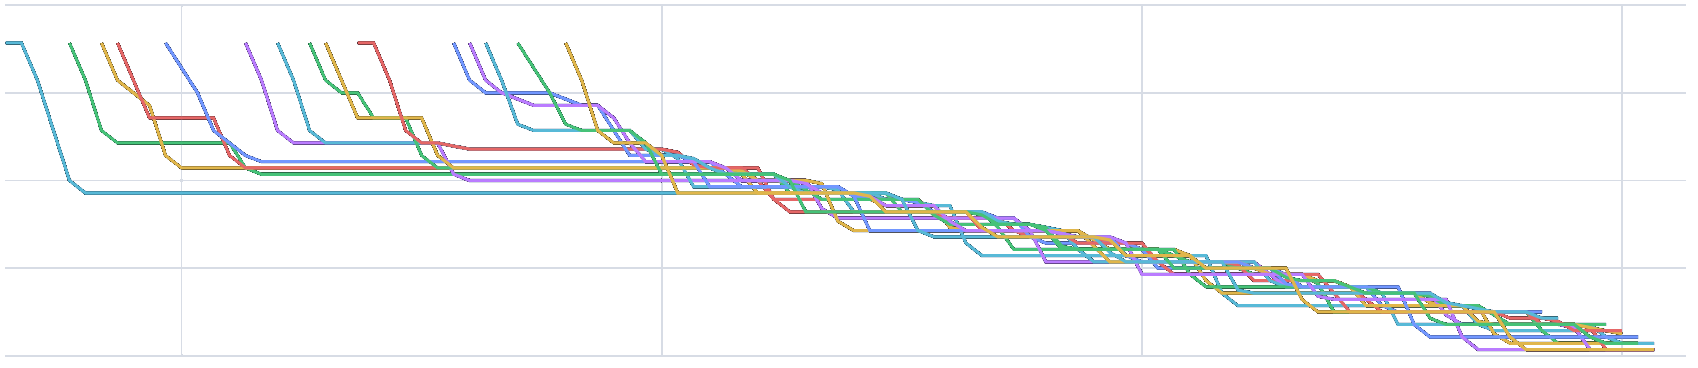
\includegraphics{images/executions/priority_alpha-inf.png}
}
\caption{
\label{priority_alpha-inf}
     Изменение приоритетов при $\alpha \to \infty$.}
\end{center}
\end{figure}

\begin{figure}[ht]
\begin{center}
\scalebox{0.3}{
   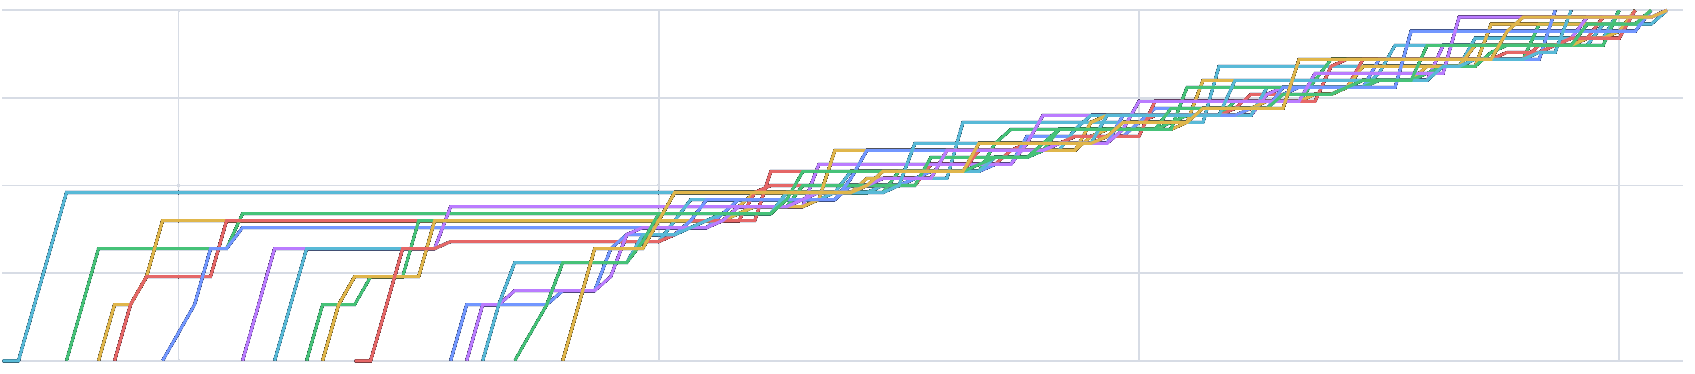
\includegraphics{images/executions/progress_alpha-inf.png}
}
\caption{
\label{progress_alpha-inf}
     Изменение прогрессов при $\alpha \to \infty$.}
\end{center}
\end{figure}

Графики, получившиеся при расчёте приоритета при учёте обоих факторов и значения $\alpha = 1$,
изображены на рисунках \ref{priority_alpha-1} и \ref{progress_alpha-1}.
Видно, что графики похожи на графики с $\alpha = 0$, но при этом можно наблюдать,
что изменения прогрессов происходят не линейно, а постепенно ступеньками,
и это означает, что планировщик чаще переключается между различными Executions, чем заканчивает исполнение очередного Execution.

\begin{figure}[ht]
\begin{center}
\scalebox{0.3}{
   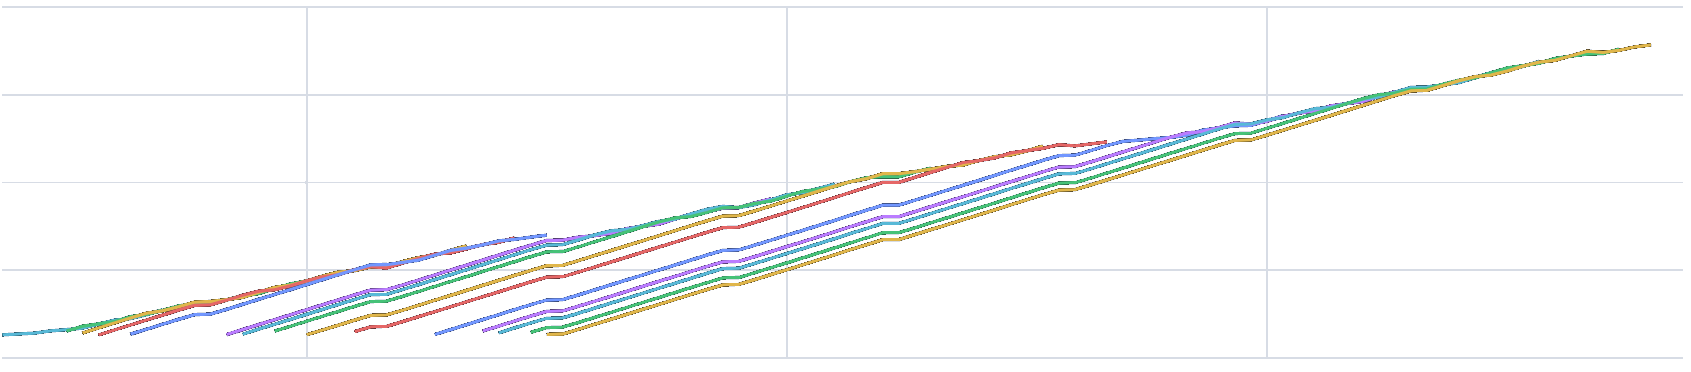
\includegraphics{images/executions/priority_alpha-1.png}
}
\caption{
\label{priority_alpha-1}
     Изменение приоритетов при $\alpha = 1$.}
\end{center}
\end{figure}

\begin{figure}[ht]
\begin{center}
\scalebox{0.3}{
   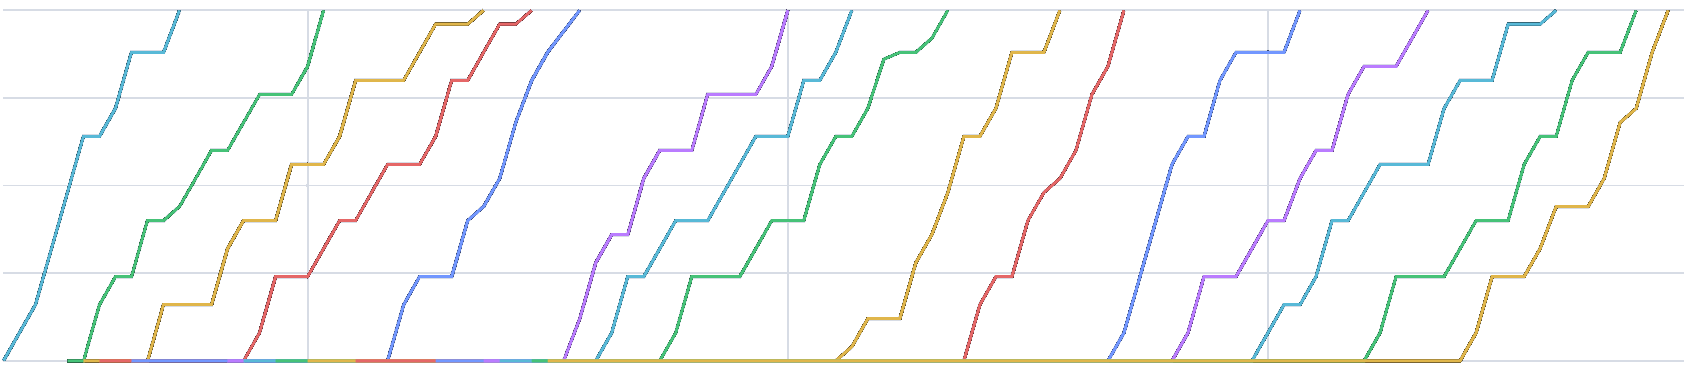
\includegraphics{images/executions/progress_alpha-1.png}
}
\caption{
\label{progress_alpha-1}
     Изменение прогрессов при $\alpha = 1$.}
\end{center}
\end{figure}

Графики, получившиеся при расчёте приоритета при учёте обоих факторов и значения $\alpha = 10$,
изображены на рисунках \ref{priority_alpha-10} и \ref{progress_alpha-10}.
Видно, что выбор Execution меняются достаточно часто, но реже, чем при $\alpha = \inf$,
и ранее появившийся Execution получает допустимое преимущество относительно более поздних Executions.

\begin{figure}[ht]
\begin{center}
\scalebox{0.3}{
   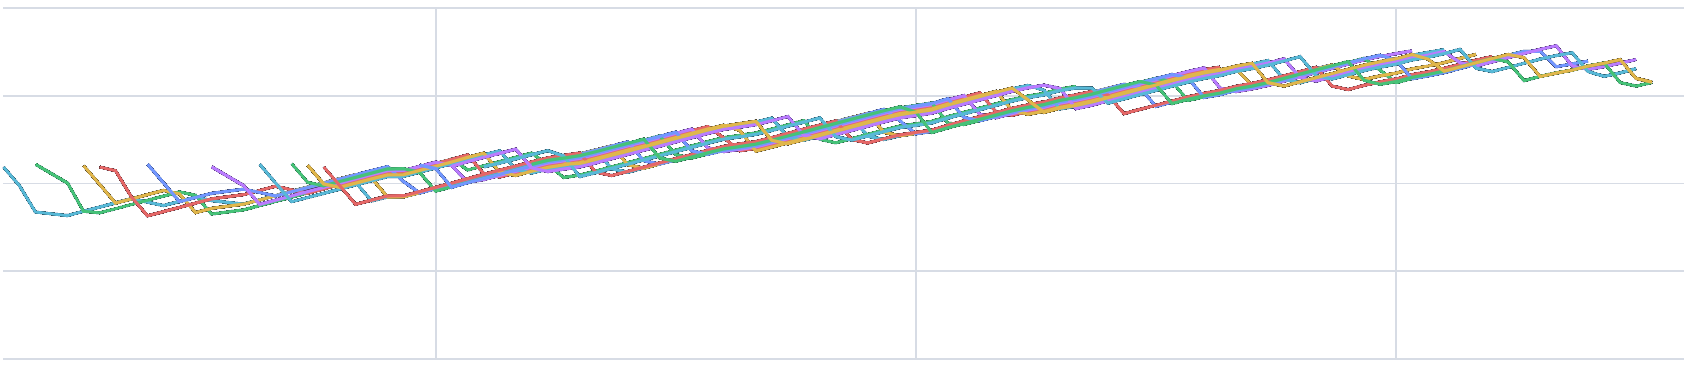
\includegraphics{images/executions/priority_alpha-10.png}
}
\caption{
\label{priority_alpha-10}
     Изменение приоритетов при $\alpha = 10$.}
\end{center}
\end{figure}

\begin{figure}[ht]
\begin{center}
\scalebox{0.3}{
   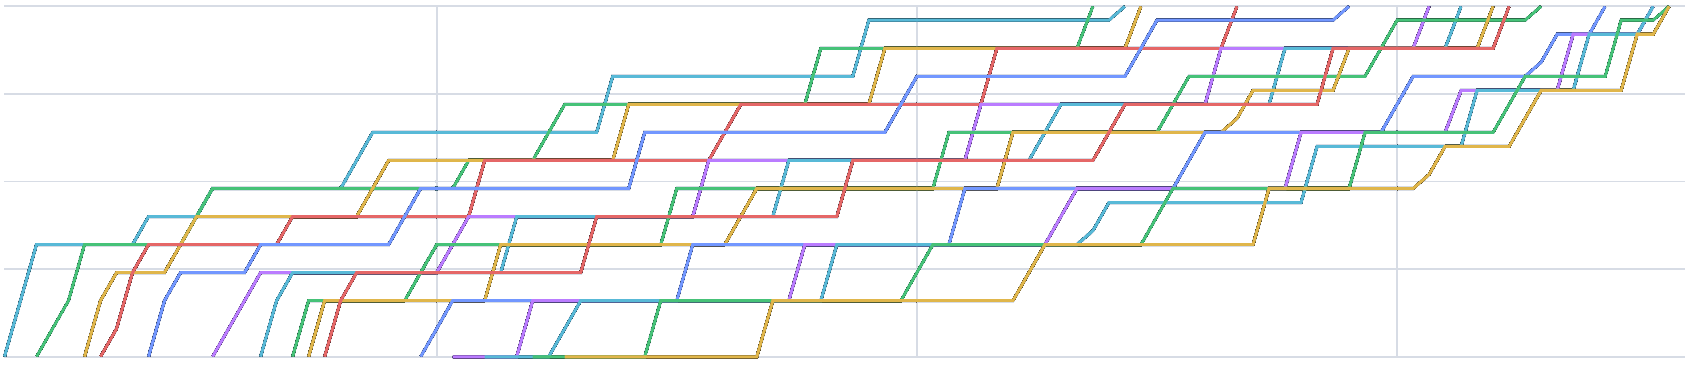
\includegraphics{images/executions/progress_alpha-10.png}
}
\caption{
\label{progress_alpha-10}
     Изменение прогрессов при $\alpha = 10$.}
\end{center}
\end{figure}

\subsubsection*{Выводы}

В ходе нагрузочного тестирования было показано,
что предложенный подход к распределению ресурсов позволяет эффективно использовать вычислительные ресурсы системы
и обеспечивает высокую степень параллельности исполнения.
Также было определено, что использование только время существования Execution приводит к эффекту застоя для новых Executions,
в то время как использование только ожидаемого оставшегося времени приводит к чрезмерно равномерному распределению ресурсов.
Наиболее сбалансированное поведение системы наблюдается при использовании комбинированной формулы приоритета,
учитывающей как время существования Execution, так и ожидаемое оставшееся время выполнения.
